
\chapter{Risultati}

Una volta completate le varie campagne di fuzzing, ognuna della durata di 36 ore, ed eseguito il processo di deduplication, ho controllato se i crash trovati fossero già noti agli sviluppatori. A tal fine ho consultato la sezione ``Issues'' dei repository GitHub dei progetti analizzati \cite{ref25}, \cite{ref26}, \cite{ref27}, \cite{ref28}.  
Per la ricerca ho usato parole chiave come l'indirizzo di crash e le prime voci della stack trace, verificando che i problemi riscontrati non fossero già segnalati.

\section{Panoramica generale}

Di seguito vengono riportati i crash riscontrati durante le campagne di fuzzing.

\begin{table}[ht]
  \centering
  \caption{Numero Crashes trovati suddivisi per programma}
  \label{tab:recap-crashes}
  \begin{tabular}{ll}
    \toprule
    \textbf{Programma} & \textbf{} \\
    \midrule
    GPAC    & 33 \\
    LibreDWG & 437 \\
    LibUCL  & 191 \\
    OpenSC  & 16 \\
    \bottomrule
  \end{tabular}
\end{table}

Osserviamo che ci sono grandi variazioni tra programmi diversi: LibreDWG è il programma che ha riscontrato più crashes in assoluto, molti però erano non riproducibili o con stack trace identica a precedenti.
Il fatto che il numero dei crashes trovato fosse così superiore agli altri non ha comportato la scoperta di un numero maggiore di bug ma semplicemente un lavoro più pesante nel processo di deduplicazione. 

Al secondo posto si colloca LibUCL, nel quale abbiamo riscontrato 191 crash, principalmente di tipo Segmentation Fault. 
Sebbene non siano errori di tipo UUM, questi crash rimangono rilevanti dal punto di vista funzionale, poiché gli input coinvolti provocano la terminazione del programma, compromettendone l’affidabilità. 

Vediamo poi GPAC, in cui abbiamo trovato un errore di tipo Conditional jump or move depends on uninitialised value, sebbene principalmente gli errori trovati fossero di tipo SEGFAULT, questi si sono risolti in seguito al github commit dello sviluppatore. 

Infine, analizziamo OpenSC all'interno del quale abbiamo trovato 16 crashes, che però si rivelano i più efficaci, infatti 3 di questi si sono rivelati unique. Due di questi coivolgono l'utilizzo di unitialized values ed uno di questi porta alla terminazione del programma. Analizziamo nella sezione Case Study - OpenSC con maggiore dettaglio questi errori.   

\subsection{OpenSC}

OpenSC è un progetto la cui finalità principale è supportare le smart card con funzioni crittografiche, vedremo più in dettaglio successivamente le sue funzionalità. 
I crash unici trovati, una volta rimossi quelli non riproducibili e quelli già reportati, per \texttt{OpenSC} sono i seguenti:

\begin{verbatim}
Use of uninitialised value of size 8
==112==    at 0x4E0C63A: _itoa_word 
==112==    by 0x4E28574: __vfprintf_internal 
==112==    by 0x4E360F8: __vsprintf_internal 

==88== Invalid read of size 1
==88==    at 0x14AD7C: asn1_encode_entry 
==88==    by 0x147671: asn1_encode 
==88==    by 0x14AC19: asn1_encode_entry 

Conditional jump or move depends on uninitialised value(s)
==118==    at 0x483FEDC: strcmp 
==118==    by 0x13B6A5: find_macro 
==118==    by 0x13B48E: build_argv 
\end{verbatim}

\subsection{LibUCL}

LibUCL è una libreria progettata per il parsing e la generazione del Universal Configuration Language (UCL), un linguaggio di configurazione orientato all’automazione e al tempo stesso leggibile da esseri umani.
I principali vantaggi offerti da UCL sono leggibilità e modificabilità manuale, con supporto ai commenti, parsabilità automatica da parte delle macchine, possibilità di conversione verso e da altri formati diffusi come YAML e JSON, supporto a macro e file di inclusione, parser estremamente veloce.

I crash unici trovati, una volta rimossi quelli non riproducibili e quelli già reportati, per \texttt{libucl} sono i seguenti:

\begin{verbatim}
==18== Invalid read of size 8
==18==    at 0x119F80: ucl_hash_destroy 
==18==    by 0x110B6F: ucl_object_free_internal 
==18==    by 0x11123D: ucl_parser_free 

==21== Invalid read of size 4
==21==    at 0x11A3E4: kh_put_ucl_hash_node
==21==    by 0x11A045: ucl_hash_insert 
==21==    by 0x10AF3D: ucl_parser_process_object_element 

==24== Invalid read of size 1
==24==    at 0x112B10: ucl_load_handler 
==24==    by 0x10DAD9: ucl_state_machine 
==24==    by 0x10C0D7: ucl_parser_add_chunk_full 
\end{verbatim}

\subsection{GPAC}

GPAC è un framework multimediale open-source, progettato con particolare attenzione alla modularità e alla conformità agli standard. Esso offre un insieme di strumenti per l’elaborazione, l’ispezione, l’impacchettamento, lo streaming, la riproduzione e l’interazione con contenuti multimediali di diversa natura.
Tali contenuti possono includere combinazioni di audio, video, sottotitoli, metadati, grafica scalabile, media cifrati, grafica 2D/3D ed ECMAScript.
GPAC è particolarmente noto per le sue avanzate capacità di gestione dei formati MP4/ISOBMFF, che lo hanno reso uno strumento di riferimento non solo per gli appassionati di video, ma anche per ricercatori accademici, enti di standardizzazione e professionisti del settore della radiodiffusione.

I crash unici trovati, una volta rimossi quelli non riproducibili e quelli già reportati, per \texttt{gpac} sono i seguenti:

\begin{verbatim}
==109== Conditional jump or move depends on uninitialised value(s)
==109==    at 0x58305C: hev_parse_vps_extension 
==109==    by 0x56D1A7: gf_hevc_read_vps_bs_internal 
==109==    by 0x570CFD: gf_hevc_parse_nalu_bs 
\end{verbatim}


\subsection{LibreDWG}

LibreDWG è una libreria C libera progettata per leggere e scrivere file nel formato DWG. Attualmente, il decoder della libreria è in grado di leggere tutte le versioni del formato DWG, con alcune limitazioni solo per oggetti avanzati introdotti a partire dalla versione R2010. Il writer, invece, supporta pienamente le versioni R1.4–R2000.

In un periodo successivo all'analisi dei crash unici trovati, abbiamo constatato che i problemi precedentemente rilevati all'aggiornamento della repository Github del progetto fossero da una parte stati corretti e dall'altra non riproducibili. 
Non abbiamo trovato quindi risultati da condividere con il relativo sviluppatore. 


\section{Case Study: OpenSC}

OpenSC fornisce un insieme di librerie e strumenti per l’interazione con smart card. L’obiettivo principale del progetto è supportare le smart card che implementano funzionalità crittografiche, favorendone l’impiego in applicazioni orientate alla sicurezza, come l’autenticazione, la cifratura della posta elettronica e la firma digitale.

L'analisi di questo programma ha rivelato 16 crashes, e in particolare 3 bug: Use of uninitialised value, Invalid read e Conditional jump or move depends on uninitialised value(s). 
Generalmente Valgrind utilizza queste diciture per indicare: 
\begin{itemize}
    \item Conditional jump or move depends on uninitialised value quando una condizione di salto o di assegnamento dipende da un valore indefinito - il comportamento del programma diventa imprevedibile;
    \item Use of unitialized value quando una funzione riceve in ingresso uno o più parametri non inizializzati, compromettendo l’esecuzione del codice all’interno della funzione stessa;
    \item Invalid Read ovvero operazioni di lettura o scrittura che superano i limiti del buffer allocato. In questo scenario, l’accesso a memoria esterna al buffer risulta pericoloso, in quanto il contenuto non è definito e può generare errori difficili da individuare.
\end{itemize}
 
\begin{figure}[htbp]        
  \centering               
  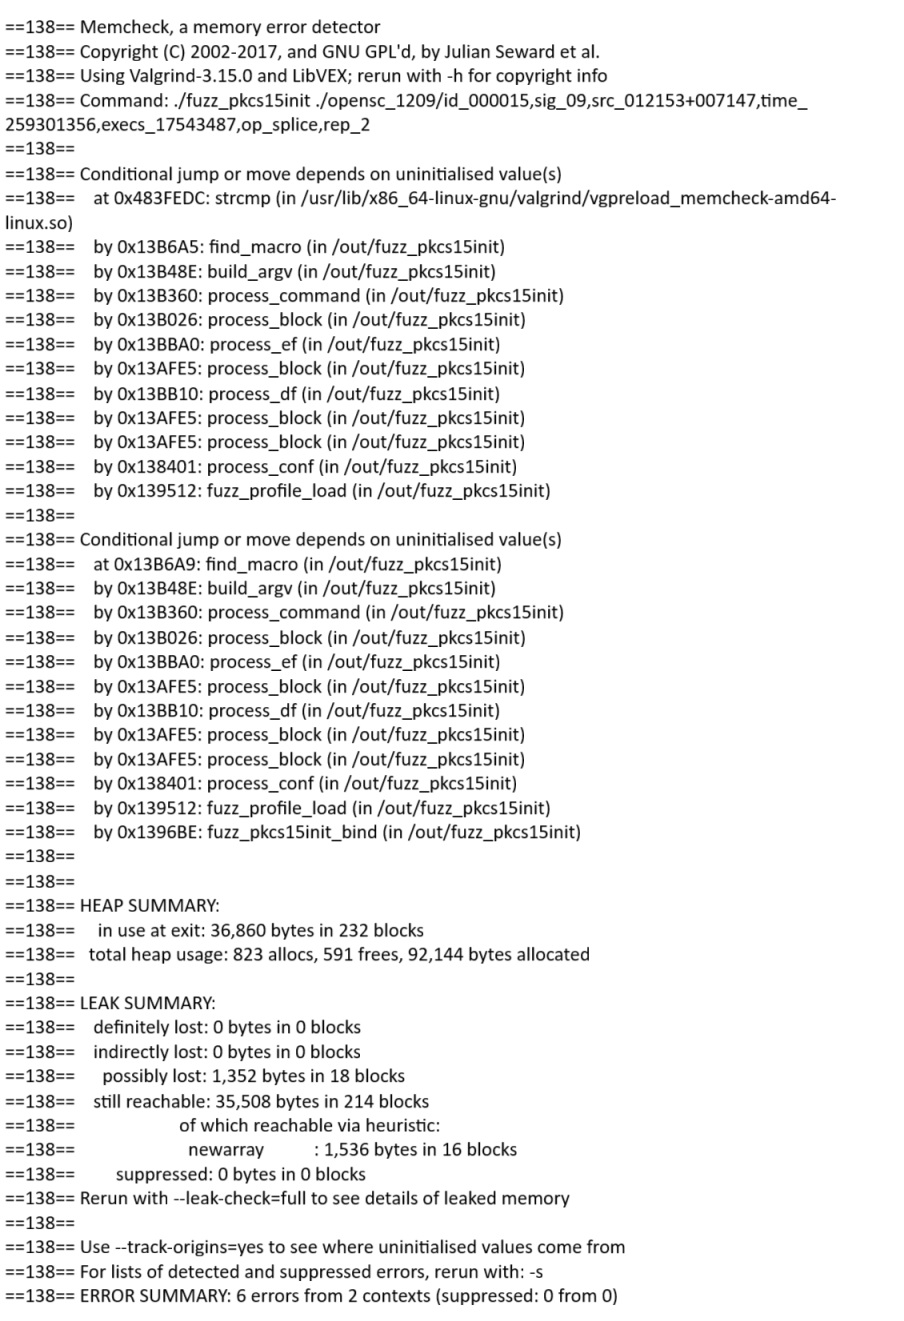
\includegraphics[width=0.7\textwidth]{immagini/valgrind-error.jpg}  
  \caption{Errore di Conditional jump su Valgrind}  
  \label{fig:valgrind-error}      
\end{figure}

Errori come gli Invalid read spesso provocano l’arresto del programma, compromettendone la funzionalità. Poiché OpenSC gestisce smart card, operazioni crittografiche e sistemi di autenticazione, la presenza di bug di memoria può avere conseguenze gravi. L’uso di memoria non inizializzata può consentire la lettura di dati sensibili già presenti (ad esempio password, chiavi o token), mentre istruzioni condizionali dipendenti da valori non inizializzati possono essere manipolate per alterare il flusso logico in modo dannoso. Di conseguenza, anche se non tutte le anomalie rilevate si traducono immediatamente in exploit, esse rappresentano comunque un rischio significativo per la sicurezza.

Gli errori trovati sono nuovi, non ancora presenti nella sezione Issues del github di OpenSC \cite{ref25}. Ci siamo inoltre assicurati che questi siano riproducibili, ovvero aggiornando l'ultimo commit disponbile questi errori sussistono. Dato quanto detto, abbiamo proceduto con la divulgazione responsabile dei suddetti \cite{ref23}.